
%(BEGIN_QUESTION)
% Copyright 2013, Tony R. Kuphaldt, released under the Creative Commons Attribution License (v 1.0)
% This means you may do almost anything with this work of mine, so long as you give me proper credit

Explain the operation of this circuit:

$$\includegraphics[width=15.5cm]{i02304x01.eps}$$


\underbar{file i02304}
%(END_QUESTION)





%(BEGIN_ANSWER)

The blue lamp will be energized whenever the pressure switch senses a pressure that is less than 45 PSI.

\vskip 10pt

The red and green lamps will both be de-energized whenever the level senses a level less than 1 foot 3 inches.  If that switch senses a level greater than 1 foot 3 inches, either the red lamp or the green lamp will energize (not both simultaneously!) based on the pressure switch's state: a pressure less than 45 PSI energizes the relay coil and energizes the green lamp, while a pressure greater than 45 PSI de-energizes the relay coil and energizes the red lamp.

%(END_ANSWER)





%(BEGIN_NOTES)

\filbreak \vskip 20pt \vbox{\hrule \hbox{\strut \vrule{} {\bf Virtual Troubleshooting} \vrule} \hrule}

\noindent
{\bf Predicting the effect of a given fault:} present each of the following faults to the students, one at a time, having them comment on all the effects each fault would produce.

\begin{itemize}
\item{} 
\item{} 
\item{} 
\end{itemize}


\vskip 10pt


\noindent
{\bf Identifying possible/impossible faults:} present symptoms to the students and then have them determine whether or not a series of suggested faults could account for all the symptoms, explaining {\it why} or {\it why not} for each proposed fault:

\begin{itemize}
\item{} Symptom: {\it Level = 2 ft and Pressure = 24 PSI; blue and red lights are energized}
\item{} Open relay contact -- {\bf No}
\item{} Open relay coil -- {\bf Yes}
\item{} Open pressure switch -- {\bf No}
\item{} Open level switch -- {\bf No}
\item{} Open fuse -- {\bf No}
\item{} Open wire between fuse and pressure switch -- {\bf No}
\item{} Open wire between relay coil and pressure switch -- {\bf Yes}
\item{} Open wire between relay coil and negative rail -- {\bf Yes}
\end{itemize}


\vskip 10pt


\noindent
{\bf Determining the utility of given diagnostic tests:} present symptoms to the students and then propose the following diagnostic tests one by one.  Students rate the value of each test, determining whether or not it would give useful information (i.e. tell us something we don't already know).  Students determine what different results for each test would indicate about the fault, if anything:

\begin{itemize}
\item{} Symptom: {\it }
\item{}  -- {\bf Yes/No}
\item{}  -- {\bf Yes/No}
\end{itemize}


\vskip 10pt


\noindent
{\bf Diagnosing a fault based on given symptoms:} imagine the ??? fails ??? in this system (don't reveal the fault to students!).  Present the operator's observation(s) to the students, have them consider possible faults and diagnostic strategies, and then tell them the results of tests they propose based on the following symptoms, until they have properly identified the nature and location of the fault:

\begin{itemize}
\item{} {\it }
\item{} 
\item{} 
\end{itemize}

%INDEX% Electronics review: electromechanical relay circuit

%(END_NOTES)


